\documentclass[11pt]{article}

\usepackage[margin=1in]{geometry}
\usepackage{graphicx}
\usepackage{booktabs}
\usepackage{float}
\usepackage{hyperref}
\usepackage{xcolor}
\usepackage{enumitem}
\usepackage{amsmath}

\graphicspath{{figures/}}

\hypersetup{
    colorlinks=true,
    linkcolor=blue,
    urlcolor=blue,
    citecolor=blue,
    pdftitle={Predicting House Sale Prices - Ames, Iowa},
    pdfauthor={Majid M. D. Ben Ghet}
}

\title{\textbf{Predicting House Sale Prices} \\ \large A Machine Learning Project on the Ames, Iowa Housing Dataset}
\author{Prepared by: Majid M. D. Ben Ghet}
\date{September 2026}

\begin{document}

\maketitle

\tableofcontents
\newpage

\section*{Executive Summary}
\addcontentsline{toc}{section}{Executive Summary}

Real estate agents and home sellers often struggle to set a fair asking price for a
house, relying mostly on gut feeling or a handful of recent comparable sales. This
project builds a machine learning model that estimates a house's sale price from its
physical characteristics, using a real dataset of 1,460 home sales in Ames, Iowa.

The raw data was riddled with short-commings such as empty cells and extreme outliers : 19 columns had missing values (some columns missing
in over 99\% of rows), a coded column was stored as a number when it should have been
treated as a category, and two clear outlier sales distorted the relationship between
living area and price. After cleaning the data, engineering a few additional
features, and comparing six regression models ranging from a simple linear baseline
to a neural network, a \textbf{Gradient Boosting} model gave the best results: it
explains about \textbf{93\%} of the variation in sale price and is typically off by
around \textbf{\$19,400}, i.e.\ roughly 1012\% of a typical house's value. The final
model is then saved and demonstrated on a handful of example houses, showing how it
could plug into a real pricing workflow.

\section{Business Understanding}

\subsection{The problem}

A real estate analytics team wants a data-driven way to estimate a \textbf{fair
listing price} for a house before it goes on the market. Today, this is largely a
manual process: an agent looks at a small number of recently sold, roughly comparable
houses and adjusts a price by feel. This works reasonably well for experienced agents
but is slow, inconsistent between agents, and easy to get wrong for unusual houses.

A price estimation model built on historical sales data would let the team:

\begin{itemize}[noitemsep]
    \item price new listings competitively as soon as a house is taken on, instead of
    waiting for a manual comparables analysis,
    \item automatically flag listings that look significantly over- or under-priced
    relative to similar houses, so an agent can double check them,
    \item give buyers and sellers an argument that is backed by facts on the price they wish to buy/sell a house for.
\end{itemize}

\subsection{Success criteria}

The model does not need to be precise with training data, house prices depend on things that are not in
this dataset at all (buyer sentiment on the day, negotiation skill, staging, and so
on). A useful model simply needs to be \textbf{close enough, consistently enough} to
be a better starting point than a rough manual estimate. As a working target, an
average error within around 10\% of a house's value would already be useful for
setting an initial asking price.

\subsection{Data source}

The dataset used for this project covers 1,460 residential home sales in Ames, Iowa,
with about 80 recorded characteristics per house  size, room counts, quality
ratings, garage and basement details, neighborhood, year built, and so on  along
with the final sale price. This is a well-known, publicly available dataset commonly
used for exactly this kind of price-prediction project.

\section{Data Understanding and Preparation}

\subsection{First look at the data}

The raw dataset has 1,460 rows and 81 columns, made up of 43 categorical (text)
columns, 35 integer columns, and 3 decimal columns. There were no duplicate rows.
Sale prices in the data range from \$34,900 to \$755,000, with a median of \$163,000
 a wide range that already hints at a right-skewed distribution, confirmed later in
the exploratory analysis.

\subsection{Missing values}

19 of the 81 columns had missing values. Figure~\ref{fig:missingness} shows the count
per column before any cleaning.

\begin{figure}[H]
    \centering
    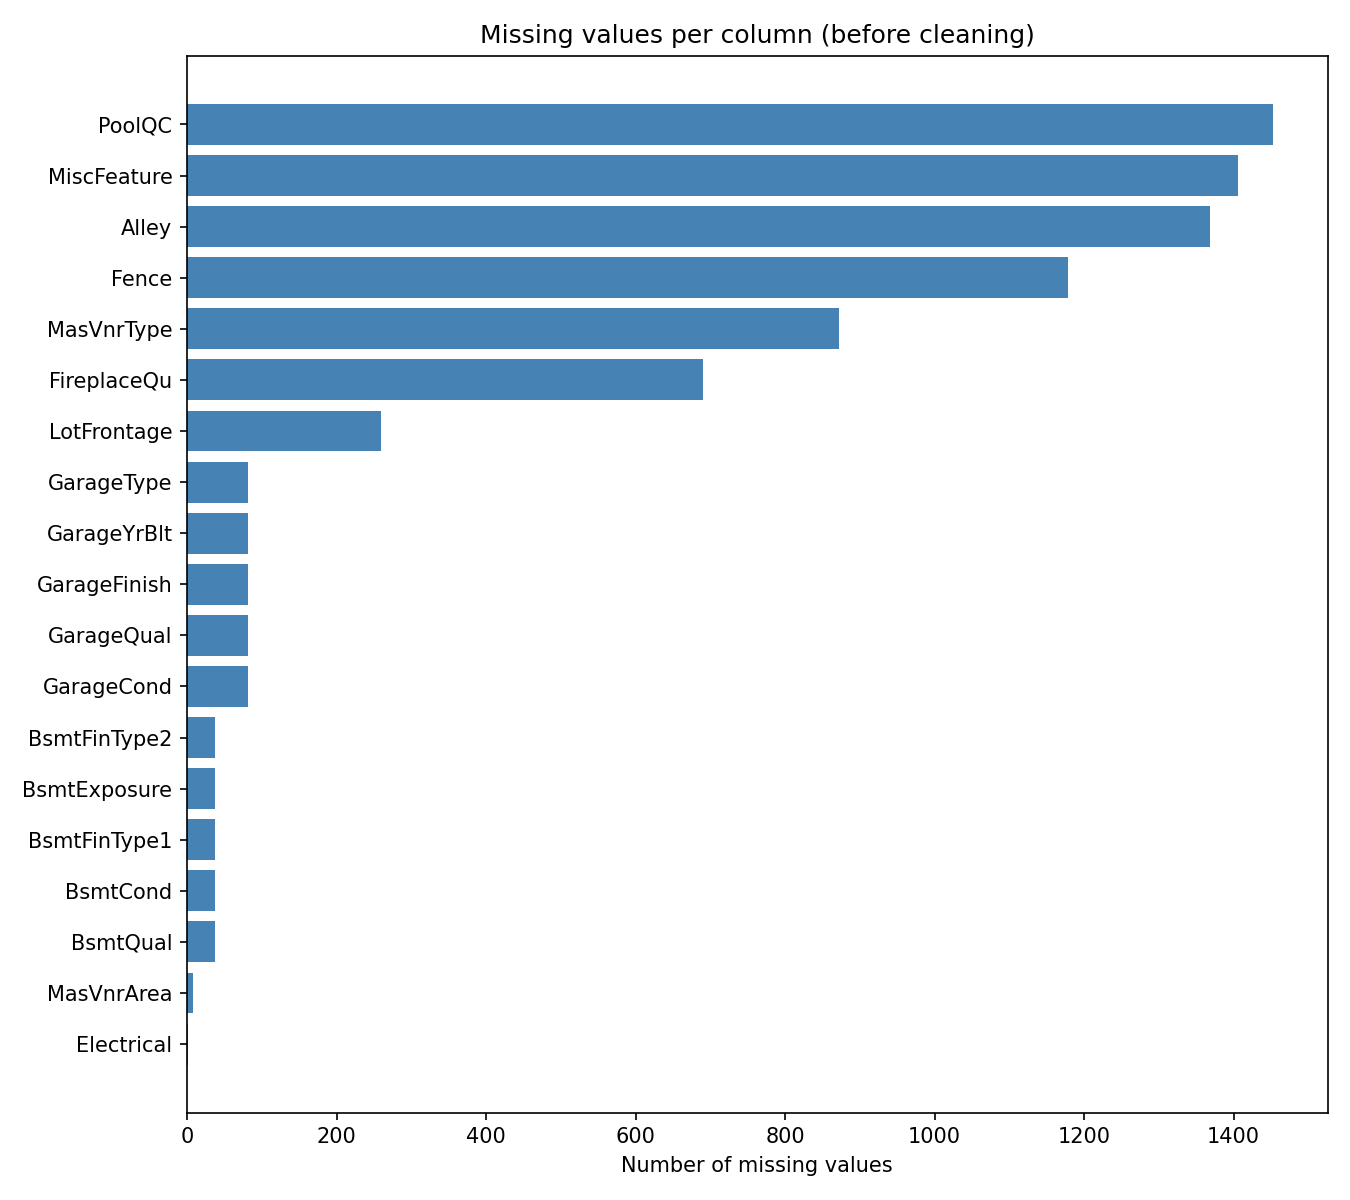
\includegraphics[width=0.85\textwidth]{fig_missingness.png}
    \caption{Missing values per column, before cleaning.}
    \label{fig:missingness}
\end{figure}

Rather than blindly dropping columns or filling every gap with a single average, each
group of missing values was handled based on what it actually means:

\begin{itemize}
    \item \textbf{``Missing'' really means ``does not have this feature.''} Columns
    like \texttt{PoolQC}, \texttt{Fence}, \texttt{FireplaceQu}, and the garage and
    basement quality/condition columns are missing precisely for houses that do not
    have a pool, fence, fireplace, garage, or basement. These were filled with the
    category \texttt{"None"} rather than treated as unknown data. This explains why
    \texttt{PoolQC} is missing in 99.5\% of rows  almost no house in the dataset has
    a pool, not because the data is broken.
    \item \textbf{\texttt{LotFrontage}} (the length of street connected to the
    property) was a genuine gap, missing for 17.7\% of houses. It was filled with the
    \textbf{median frontage of houses in the same neighborhood}, since lot sizes tend
    to be similar within a neighborhood, rather than a single dataset-wide average.
    \item \textbf{\texttt{GarageYrBlt}} and \textbf{\texttt{MasVnrArea}} were filled
    with 0, since a missing value here almost always means there is no garage or no
    masonry veneer.
    \item \textbf{\texttt{Electrical}} had exactly one missing value out of 1,460, so
    it was filled with the single most common electrical system in the dataset.
\end{itemize}

After these steps, the dataset had zero remaining missing values.

\subsection{A data type correction}

\texttt{MSSubClass} is stored as a number (20, 60, 120, \ldots) but is actually a
coded category  for example, 20 represents a 1-story house built after 1946, while
60 represents a 2-story house built after 1946. Left as a number, a model would
wrongly treat a higher code as ``more'' of something. This column was converted to
text so that it is correctly treated as a category.

\subsection{Outliers}

Figure~\ref{fig:outliers} plots living area against sale price before cleaning. Two
houses stand out clearly: both have an unusually large living area (over 4,000 square
feet) but sold for a surprisingly low price (under \$300,000), well below what their
size would suggest. These are almost certainly unusual sales rather than typical
market transactions, and were removed, leaving 1,458 rows.

\begin{figure}[H]
    \centering
    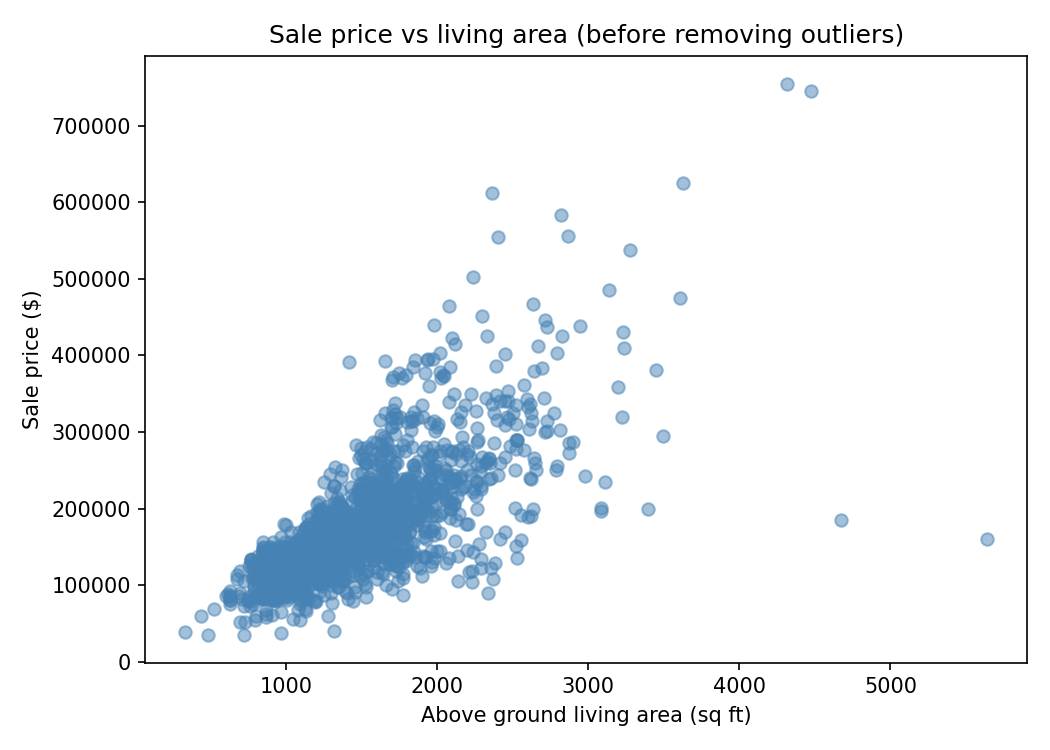
\includegraphics[width=0.7\textwidth]{fig_outliers_before.png}
    \caption{Sale price vs.\ living area before removing outliers. The two points in
    the bottom right are the removed outliers.}
    \label{fig:outliers}
\end{figure}

\subsection{Feature engineering}

Four additional columns were built from existing ones, all fairly standard for a
housing dataset:

\begin{itemize}[noitemsep]
    \item \textbf{TotalSF}  total finished square footage (basement + first floor +
    second floor)
    \item \textbf{HouseAge}  the age of the house in the year it was sold
    \item \textbf{RemodeledFlag}  whether the house was ever remodeled
    \item \textbf{TotalBath}  total number of bathrooms, counting half-bathrooms as
    0.5
\end{itemize}

After cleaning and feature engineering, the dataset used for modeling has 39 numeric
columns and 44 categorical columns.

\subsection{Exploratory analysis}

The sale price itself is right-skewed: most houses sell in a fairly typical range, but
a smaller number of expensive houses stretch the distribution's tail out to the
right. Taking the log of the price makes the distribution far more symmetric
(Figure~\ref{fig:target-dist}), so \textbf{the models in this project were trained to
predict log(sale price)}, with predictions converted back to dollars afterward. This
is a standard trick that generally helps models  especially linear ones  avoid
being thrown off by a handful of very expensive houses.

\begin{figure}[H]
    \centering
    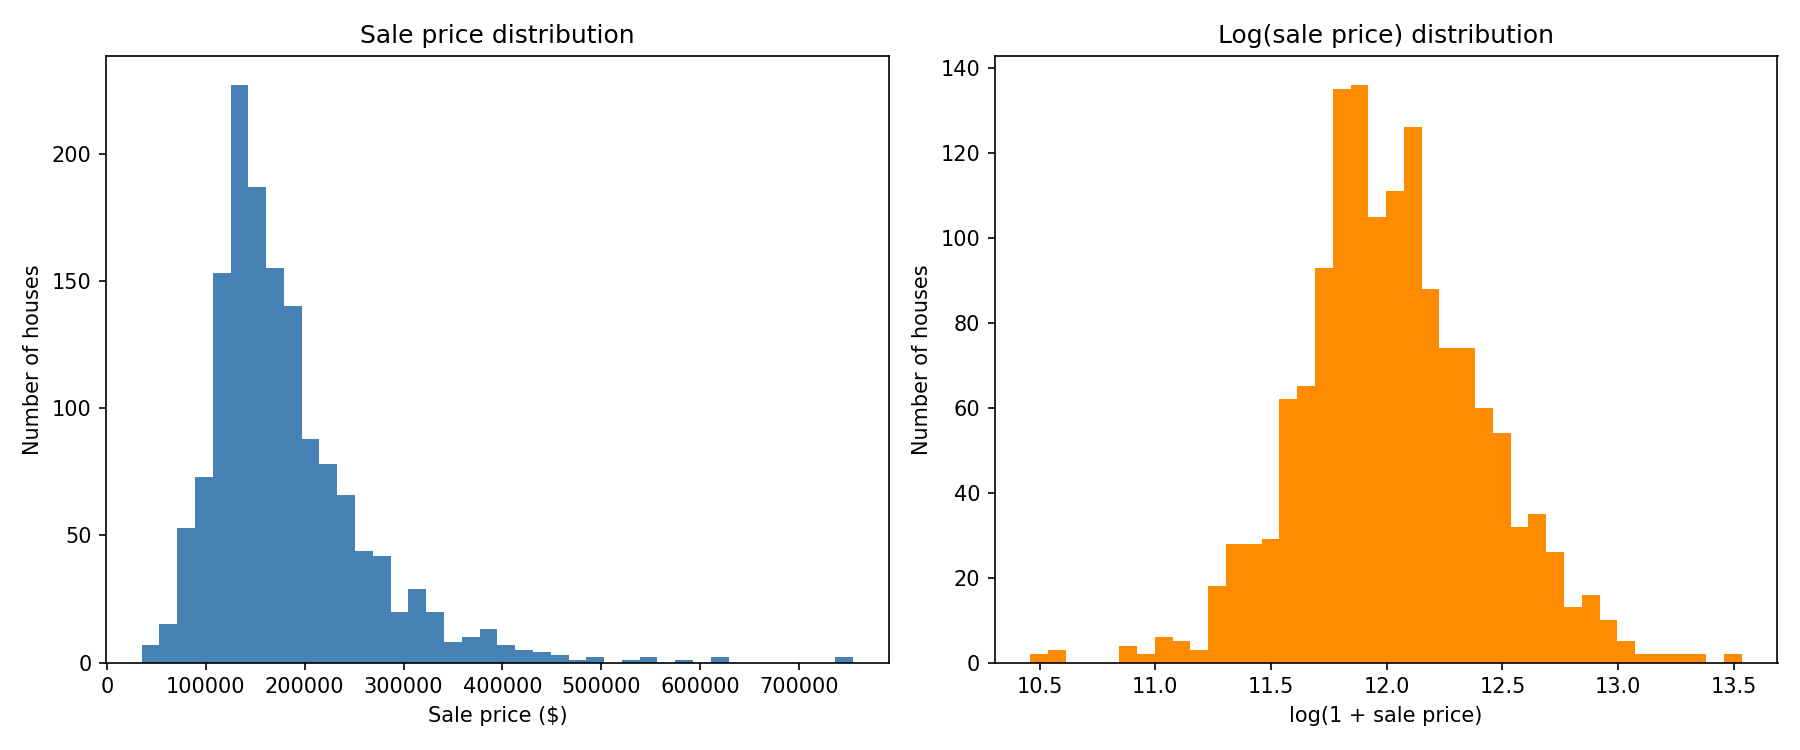
\includegraphics[width=\textwidth]{fig_target_dist.png}
    \caption{Sale price distribution (left) and log(sale price) distribution
    (right).}
    \label{fig:target-dist}
\end{figure}

Table~\ref{tab:correlations} lists the numeric features most strongly correlated with
sale price. Total square footage, overall quality, and living area top the list 
all things that match common sense about what drives a house's value.

\begin{table}[H]
    \centering
    \caption{Numeric features most correlated with sale price.}
    \label{tab:correlations}
    \begin{tabular}{lc}
        \toprule
        \textbf{Feature} & \textbf{Correlation with SalePrice} \\
        \midrule
        TotalSF (engineered)      & 0.833 \\
        OverallQual                & 0.796 \\
        GrLivArea                  & 0.735 \\
        TotalBsmtSF                & 0.651 \\
        GarageCars                 & 0.641 \\
        TotalBath (engineered)     & 0.636 \\
        1stFlrSF                   & 0.632 \\
        GarageArea                 & 0.629 \\
        FullBath                   & 0.562 \\
        TotRmsAbvGrd                & 0.538 \\
        \bottomrule
    \end{tabular}
\end{table}

\begin{figure}[H]
    \centering
    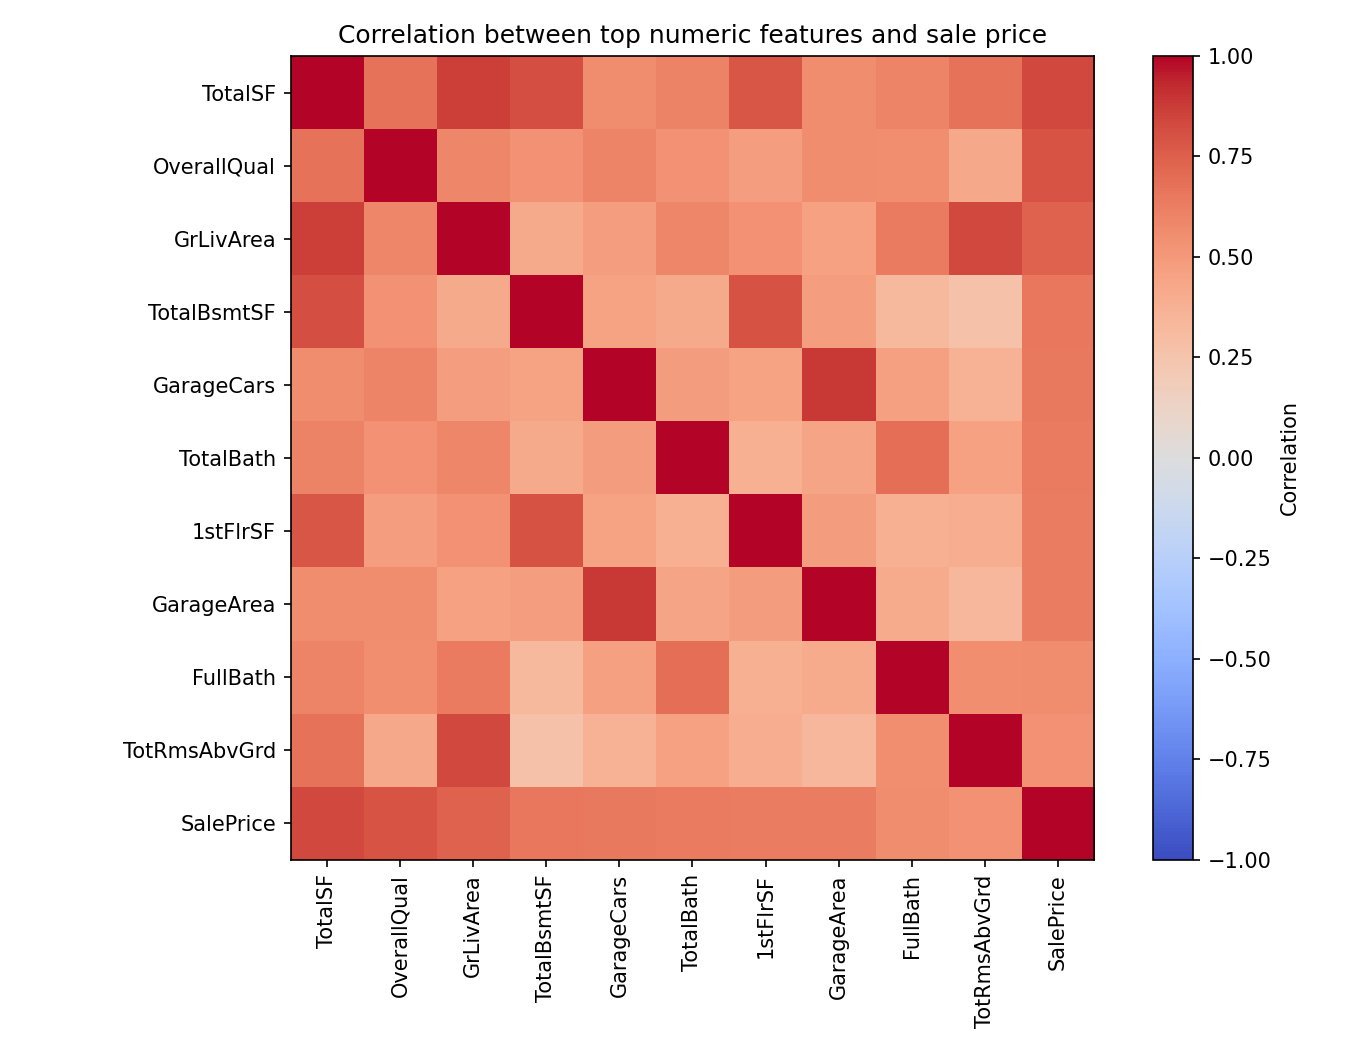
\includegraphics[width=0.75\textwidth]{fig_corr_heatmap.png}
    \caption{Correlation between the top numeric features and sale price.}
    \label{fig:heatmap}
\end{figure}

Two categorical relationships stood out clearly during the exploration. Sale price
varies a great deal by neighborhood (Figure~\ref{fig:neighborhood}), and rises in an
almost step-like way with the overall quality rating (Figure~\ref{fig:quality}) 
both good signs that the target has a strong, learnable relationship with features the
model has access to.

\begin{figure}[H]
    \centering
    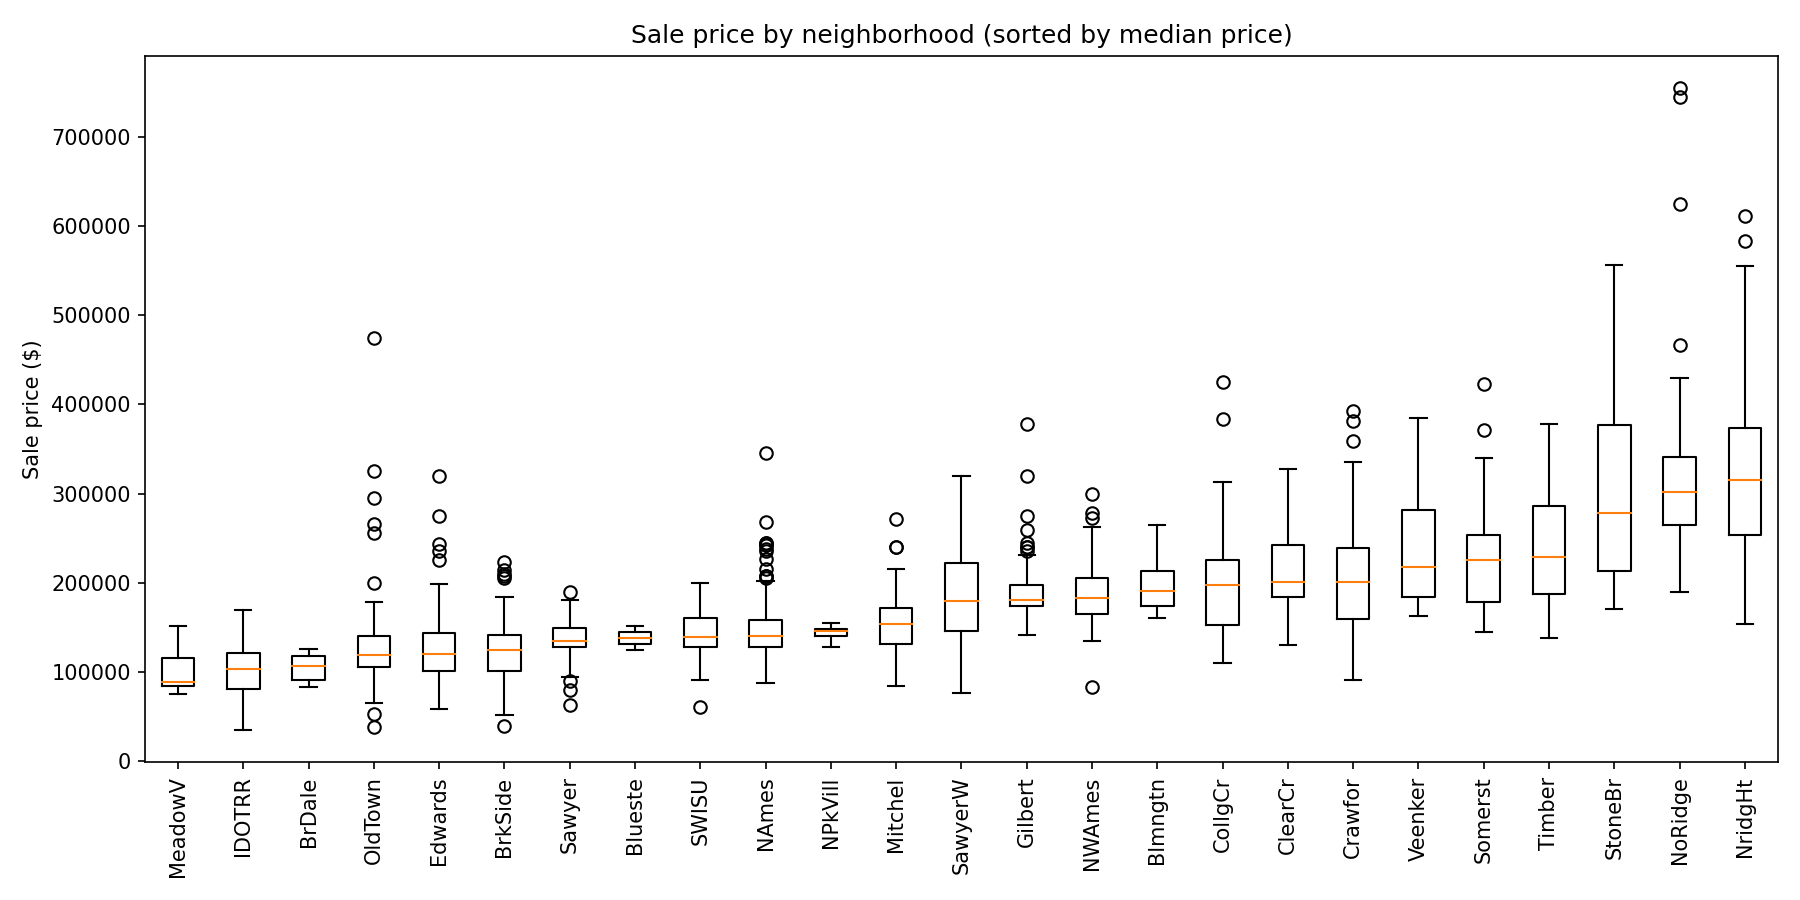
\includegraphics[width=\textwidth]{fig_boxplot_neighborhood.png}
    \caption{Sale price by neighborhood, sorted by median price.}
    \label{fig:neighborhood}
\end{figure}

\begin{figure}[H]
    \centering
    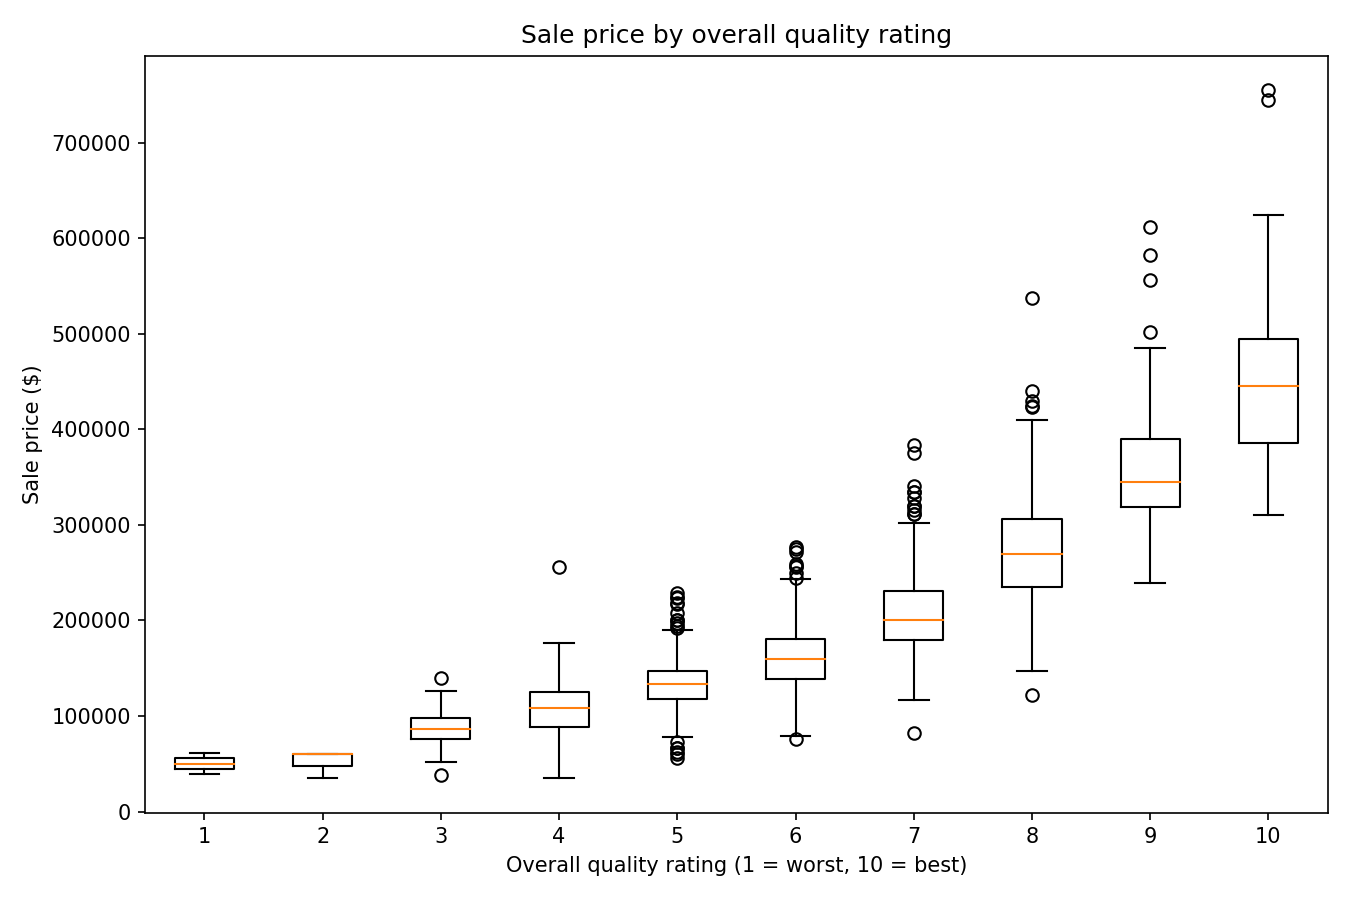
\includegraphics[width=0.8\textwidth]{fig_boxplot_quality.png}
    \caption{Sale price by overall quality rating (1 = worst, 10 = best).}
    \label{fig:quality}
\end{figure}

\section{Modeling}

\subsection{Preprocessing pipeline}

Before any model can be trained, the data needs a consistent set of preprocessing
steps:

\begin{itemize}[noitemsep]
    \item a safety-net imputer to fill any unexpected remaining gaps,
    \item scaling for numeric columns, so that features on very different scales
    (square footage vs.\ a 110 rating) do not unfairly dominate the linear and
    neural network models,
    \item one-hot encoding for categorical columns (like \texttt{Neighborhood}),
    since models cannot work with text directly.
\end{itemize}

These steps were combined into a single scikit-learn \texttt{ColumnTransformer},
wrapped in a \texttt{Pipeline} together with each model. This guarantees the exact
same transformation is applied to training data, test data, and any new data used
later for predictions.

\subsection{Train/test split}

The data was split 80/20 into a training set (1,166 houses) and a held-out test set
(292 houses), with a fixed random seed so results are reproducible.

\subsection{Hyperparameter tuning}

Before the final model comparison, a small grid search was run on the Random Forest to
check whether a bigger forest or deeper trees make a meaningful difference. The
search covered \texttt{n\_estimators} $\in \{100, 300\}$ and \texttt{max\_depth} $\in
\{10, \text{None}\}$ with 3-fold cross-validation. The best combination
(\texttt{n\_estimators=300}, \texttt{max\_depth=None}) was carried forward into the
main comparison below. The search was kept intentionally small  the goal was to
demonstrate the tuning process, not to exhaustively search every possible setting.

\subsection{Models compared}

Six regression models were compared, chosen to span a range from very simple to more
advanced, so the analysis shows whether the added complexity of an ensemble or a
neural network actually pays off on this problem:

\begin{itemize}
    \item \textbf{Linear Regression}  the simplest possible baseline. Assumes a
    straight-line relationship between the features and price, with no
    regularization.
    \item \textbf{Ridge Regression}  a linear model with an added penalty on large
    coefficients. Chosen specifically because the one-hot encoded categorical columns
    create a lot of correlated, sometimes redundant features, which plain linear
    regression handles poorly (see Section~\ref{sec:linreg-instability}).
    \item \textbf{Decision Tree}  captures non-linear relationships and feature
    interactions that a linear model cannot, while still being fairly easy to
    interpret.
    \item \textbf{Random Forest}  an ensemble of many decision trees trained on
    random subsets of the data and features. Generally more accurate and more stable
    than any single tree.
    \item \textbf{Gradient Boosting}  another tree ensemble, but one that builds
    trees sequentially, with each new tree correcting the mistakes of the ones before
    it. Often the strongest performer on structured, tabular data like this.
    \item \textbf{Neural Network (Multi-Layer Perceptron)}  included as the more
    advanced, ``modern'' model. Neural networks typically need substantially more
    data and more careful tuning to outperform tree ensembles on a tabular dataset
    this size (under 1,500 rows), so it was included as much for comparison as for
    raw accuracy.
\end{itemize}

Each model was trained inside the same preprocessing pipeline, evaluated on the held-out
test set, and cross-validated with 5-fold cross-validation on the training set as an
additional stability check.

\section{Evaluation}

\subsection{Model comparison}

Table~\ref{tab:results} summarizes the results for all six models. Root Mean Squared
Error (RMSE) and Mean Absolute Error (MAE) are both reported in dollars (lower is
better); R\textsuperscript{2} indicates the proportion of variation in price the model
explains (closer to 1 is better).

\begin{table}[H]
    \centering
    \caption{Test-set performance of all six models.}
    \label{tab:results}
    \begin{tabular}{lrrr}
        \toprule
        \textbf{Model} & \textbf{RMSE (\$)} & \textbf{MAE (\$)} & \textbf{R\textsuperscript{2}} \\
        \midrule
        Linear Regression   & 550,043.55 & 72,226.01 & $-53.77$ \\
        Ridge Regression    & 20,128.97  & 14,346.88 & 0.927 \\
        Decision Tree       & 43,613.05  & 28,019.57 & 0.656 \\
        Random Forest       & 23,453.12  & 16,278.07 & 0.900 \\
        \textbf{Gradient Boosting} & \textbf{19,393.14} & \textbf{13,894.54} & \textbf{0.932} \\
        Neural Network (MLP) & 37,869.83 & 23,326.46 & 0.740 \\
        \bottomrule
    \end{tabular}
\end{table}

\textbf{Gradient Boosting} came out on top, explaining about 93\% of the variation in
sale price with a typical error of roughly \$19,400. Random Forest and Ridge
Regression were close behind. Figure~\ref{fig:comparison} shows the same comparison
visually (Linear Regression is excluded from the chart  see the note below  since
its error is orders of magnitude larger and would make the other bars unreadable).

\begin{figure}[H]
    \centering
    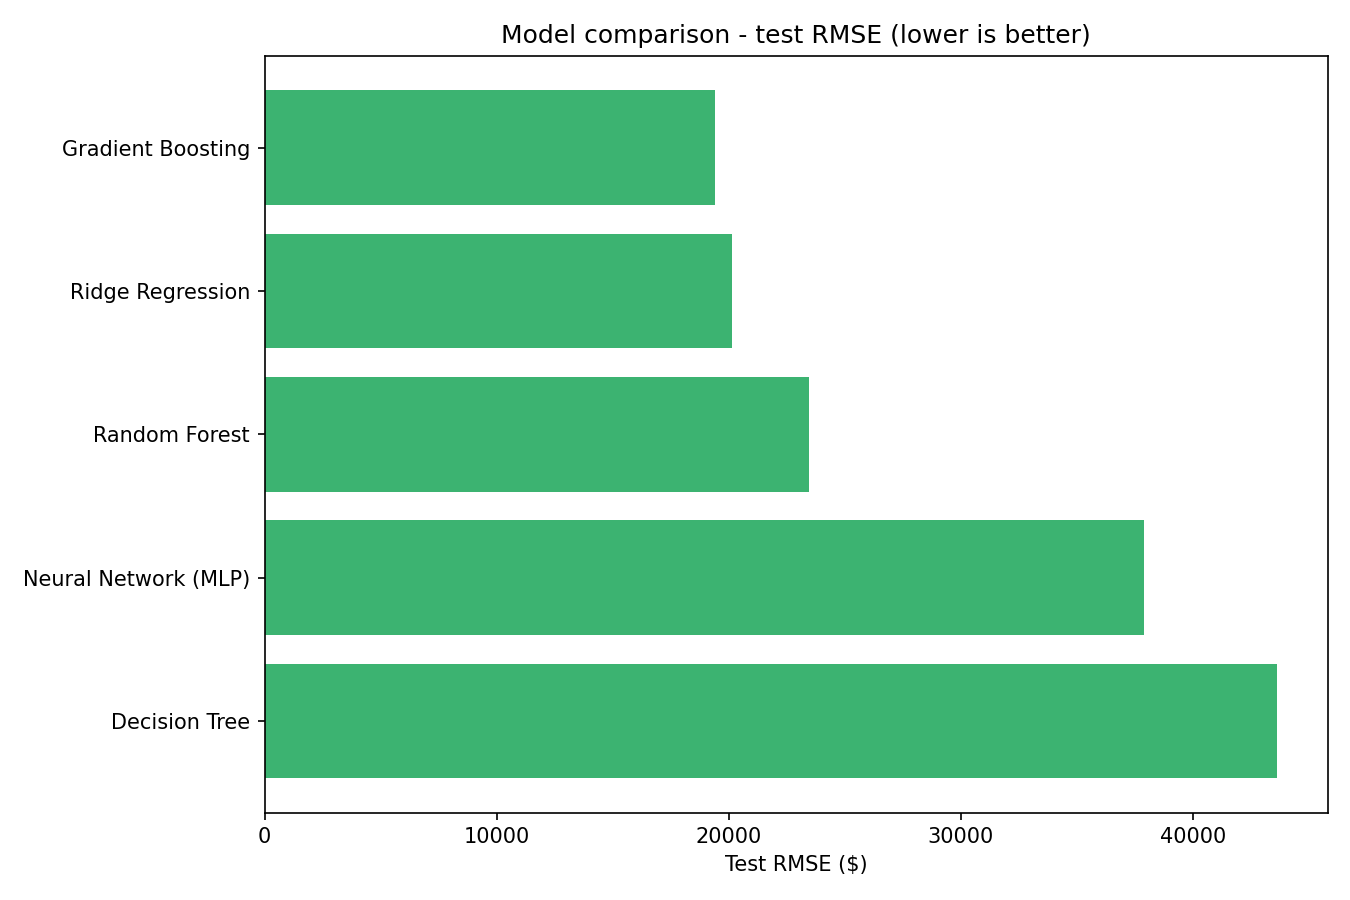
\includegraphics[width=0.8\textwidth]{fig_model_comparison.png}
    \caption{Test RMSE by model (lower is better). Linear Regression omitted; see
    Section~\ref{sec:linreg-instability}.}
    \label{fig:comparison}
\end{figure}

\subsubsection{Why did plain Linear Regression fail so badly?}
\label{sec:linreg-instability}

Linear Regression's result (RMSE of \$550,043 and a strongly negative
R\textsuperscript{2}) is not a bug  it is a real, and fairly common, failure mode.
After one-hot encoding, the dataset has around 300 columns, several of which
correspond to rare category levels that appear only once or twice in the 1,166-row
training set. With that many columns relative to that few rows, plain unregularized
linear regression becomes numerically unstable and produces a handful of wildly
unrealistic predictions, which dominate the error metrics.

This is exactly the textbook argument for regularization. Ridge Regression uses the
identical features and preprocessing, but adds a penalty that discourages excessively
large coefficients  and its RMSE of \$20,129 (versus \$550,043) shows just how
completely that fixes the problem. This result is included in the report deliberately,
as a useful, concrete illustration of why regularization matters, rather than smoothed
over.

\subsection{Understanding the best model}

\subsubsection{Which features matter most?}

Tree-based models can report which features they relied on most when making
predictions. Figure~\ref{fig:importance} shows the top 20 features for the winning
Gradient Boosting model. Total square footage and overall quality rating dominate,
together accounting for the large majority of the model's decision-making, which lines
up well with the correlations found during exploratory analysis.

\begin{figure}[H]
    \centering
    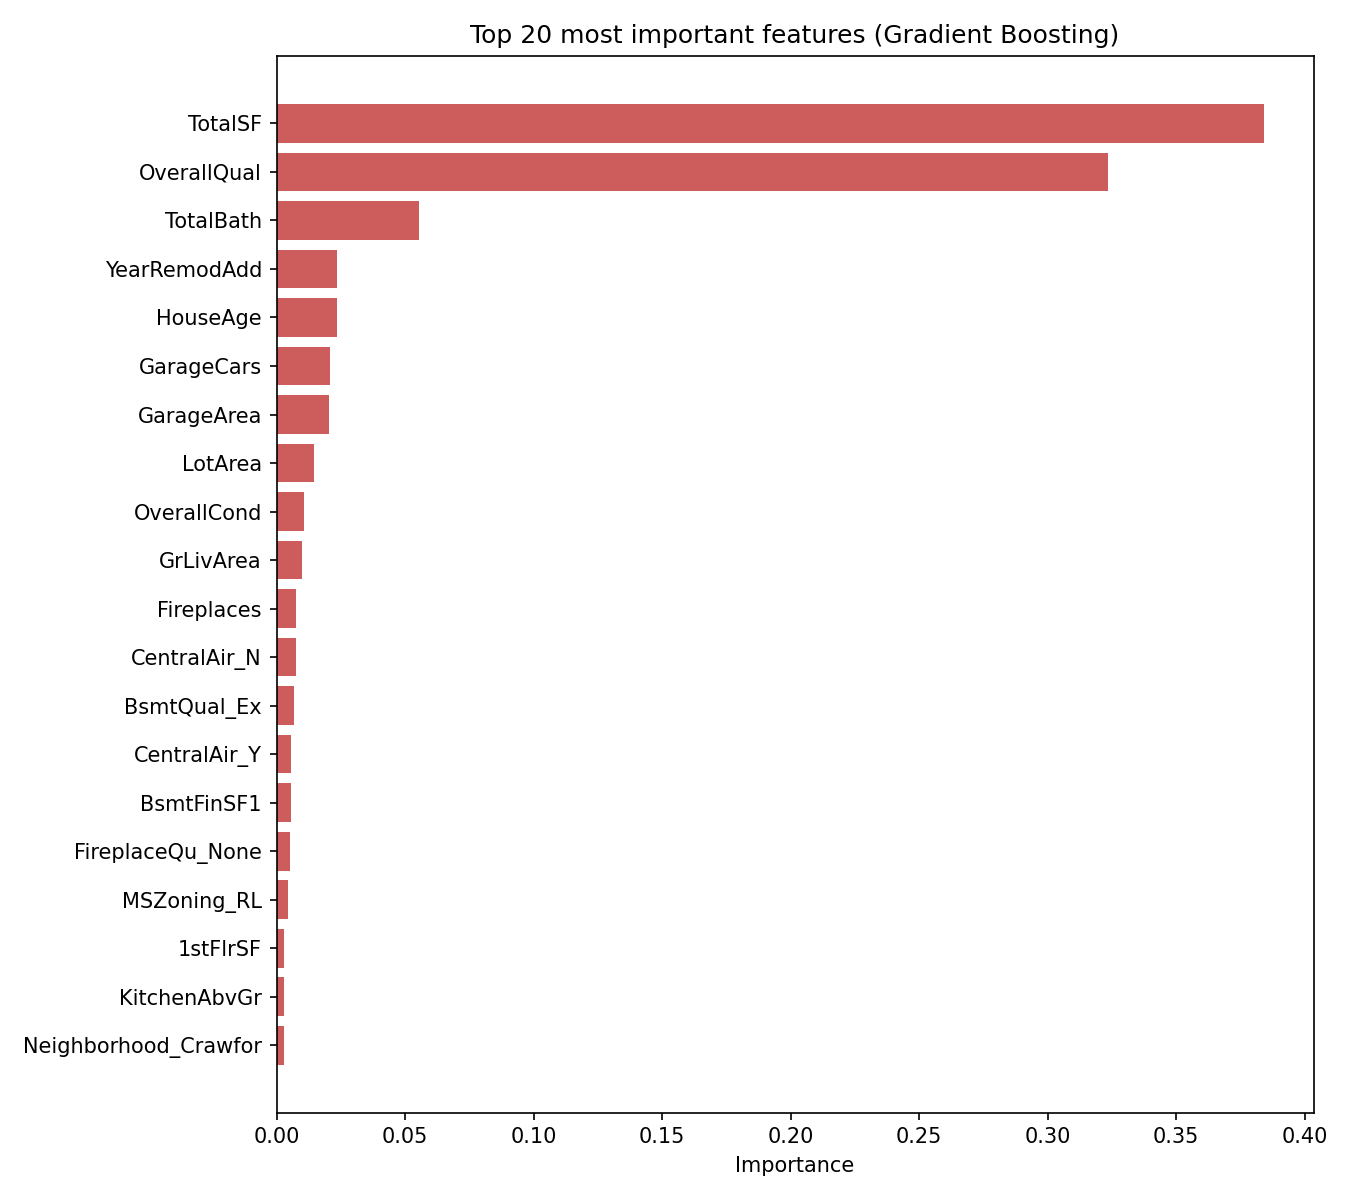
\includegraphics[width=0.85\textwidth]{fig_feature_importance.png}
    \caption{Top 20 most important features for the Gradient Boosting model.}
    \label{fig:importance}
\end{figure}

\subsubsection{Predicted vs.\ actual price, and residuals}

Figure~\ref{fig:pred-vs-actual} plots predicted price against actual price for every
house in the test set; a perfect model would place every point exactly on the red
diagonal line. Most points sit close to that line, though the model's errors grow
somewhat for the most expensive houses  there are fewer of those in the training
data for the model to learn from.

\begin{figure}[H]
    \centering
    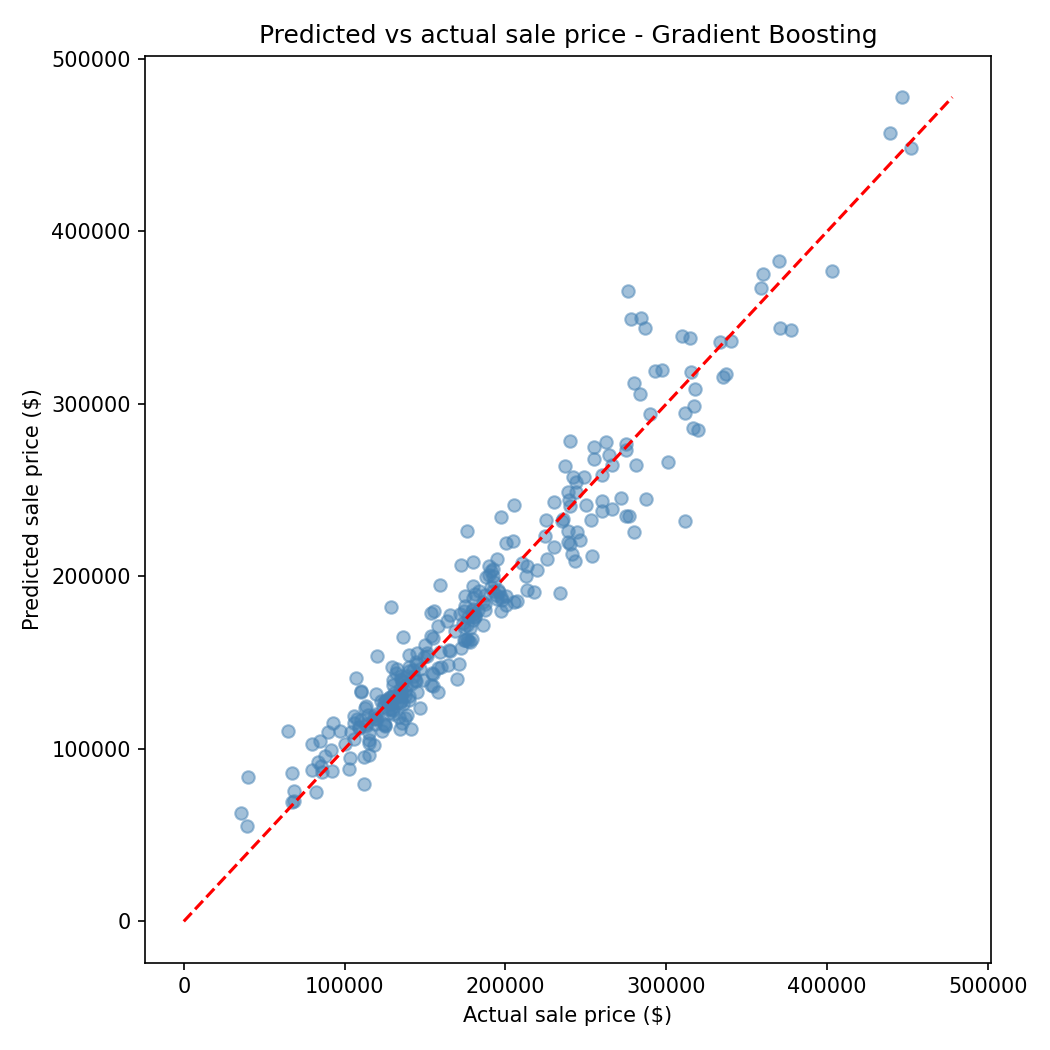
\includegraphics[width=0.6\textwidth]{fig_pred_vs_actual.png}
    \caption{Predicted vs.\ actual sale price on the test set (Gradient Boosting).}
    \label{fig:pred-vs-actual}
\end{figure}

Figure~\ref{fig:residuals} shows the distribution of residuals (actual price minus
predicted price). The errors are roughly centered on zero and reasonably symmetric,
with a small number of larger errors  mostly the same expensive houses visible in
Figure~\ref{fig:pred-vs-actual}.

\begin{figure}[H]
    \centering
    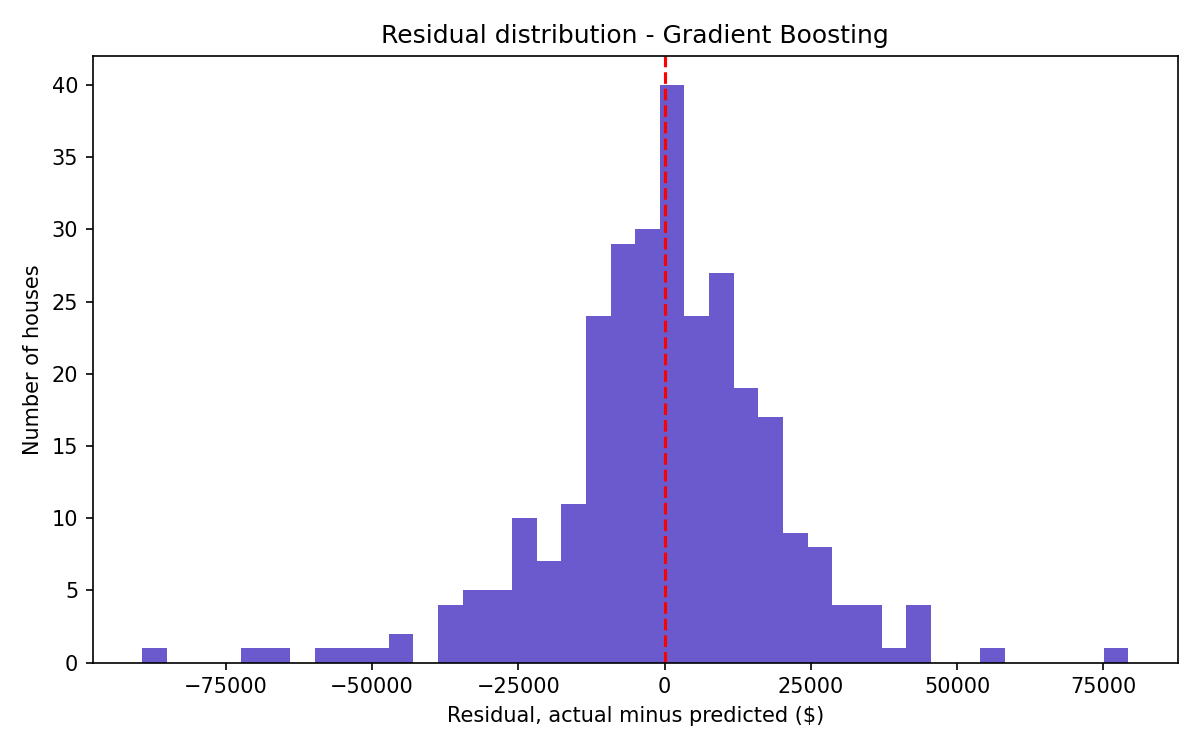
\includegraphics[width=0.65\textwidth]{fig_residuals.png}
    \caption{Residual distribution on the test set (Gradient Boosting).}
    \label{fig:residuals}
\end{figure}

\subsection{Accuracy vs.\ interpretability}

It is worth being explicit about the trade-off between the models compared. Ridge
Regression, despite being much simpler than Gradient Boosting, came within about
\$700 of it on RMSE, and a linear model's coefficients are far easier to explain to a
non-technical stakeholder (``each additional bathroom adds roughly \$X to the
estimate'') than a boosted tree ensemble's internal logic. If interpretability mattered
more than squeezing out the last few percent of accuracy, Ridge Regression would be a
very reasonable choice. Gradient Boosting was selected here because raw accuracy was
prioritized, but this trade-off would be worth revisiting with the business
stakeholders in a real deployment.

\section{Deployment}

A prediction model is only useful if it can be reused without re-running the entire
analysis every time. The final, fitted Gradient Boosting pipeline  including every
preprocessing step  was saved to disk using \texttt{joblib}, so it can be loaded and
used independently of this notebook.

To confirm the saved pipeline works correctly, it was reloaded and used to predict
prices for five houses from the test set that the model had not seen during training.
Table~\ref{tab:deployment} shows the results.

\begin{table}[H]
    \centering
    \caption{Example predictions from the saved, reloaded pipeline.}
    \label{tab:deployment}
    \begin{tabular}{lrrr}
        \toprule
        \textbf{House} & \textbf{Actual price} & \textbf{Predicted price} & \textbf{Difference} \\
        \midrule
        1320 & \$190,000 & \$206,235 & +\$16,235 \\
        836  & \$100,000 & \$103,046 & +\$3,046 \\
        413  & \$115,000 & \$109,408 & $-$\$5,592 \\
        522  & \$159,000 & \$156,287 & $-$\$2,713 \\
        1035 & \$315,500 & \$318,376 & +\$2,876 \\
        \bottomrule
    \end{tabular}
\end{table}

All five predictions land within about \$16,000 of the actual sale price, and four of
the five are within \$6,000  a solid result for an automated first estimate.

In a real deployment, this saved pipeline is the piece that would sit behind a simple
internal tool: an agent enters a house's details into a form, and the tool loads the
pipeline and returns a price estimate in well under a second. Because the
preprocessing steps are saved as part of the same pipeline object, new data does not
need to be manually cleaned or encoded before predicting  the pipeline handles that
automatically, provided the input has the same columns as the training data. Turning
this into an actual internal tool (for example, a small web form) was left out of
scope here, but would be a natural next step.

\section{Conclusion and Limitations}

Starting from a real, messy dataset with genuine missing values, a mismatched data
type, and clear outliers, this project cleaned the data, engineered a handful of
useful features, and compared six regression models ranging from a plain linear
baseline to a neural network. The tree-based ensembles  Random Forest and especially
Gradient Boosting  gave the strongest results, comfortably beating the unregularized
linear baseline (which turned out to be numerically unstable given the number of
one-hot encoded columns) and modestly outperforming both Ridge Regression and the
neural network.

\textbf{Limitations:}
\begin{itemize}
    \item The dataset covers only Ames, Iowa, and only sales from a specific historical
    period. The model would need to be retrained, or at least re-validated, before
    being used in a different market or after enough time has passed for prices to
    have shifted meaningfully.
    \item The model's errors grow for the most expensive houses, simply because there
    are fewer of them in the training data.
    \item Hyperparameter tuning was intentionally kept light. A more exhaustive
    search  particularly for the neural network, which likely needs more tuning to
    reach its full potential  could close some of the remaining performance gap.
\end{itemize}

\textbf{Possible next steps:} collecting more recent sales data (including sales from
other cities, to make the model more broadly usable), running a wider
hyperparameter search, and wrapping the saved pipeline in a simple internal web tool
would all be natural ways to move this from a working prototype toward something an
agent could use day to day.

\appendix
\section{Appendix: Additional Context}

\subsection{Living area vs. price, after cleaning}

Figure~\ref{fig:grlivarea-after} shows the same living-area-vs-price relationship as
Figure~\ref{fig:outliers}, after the two outlier houses were removed. The relationship
is much cleaner and more consistent once those two unusual sales are gone.

\begin{figure}[H]
    \centering
    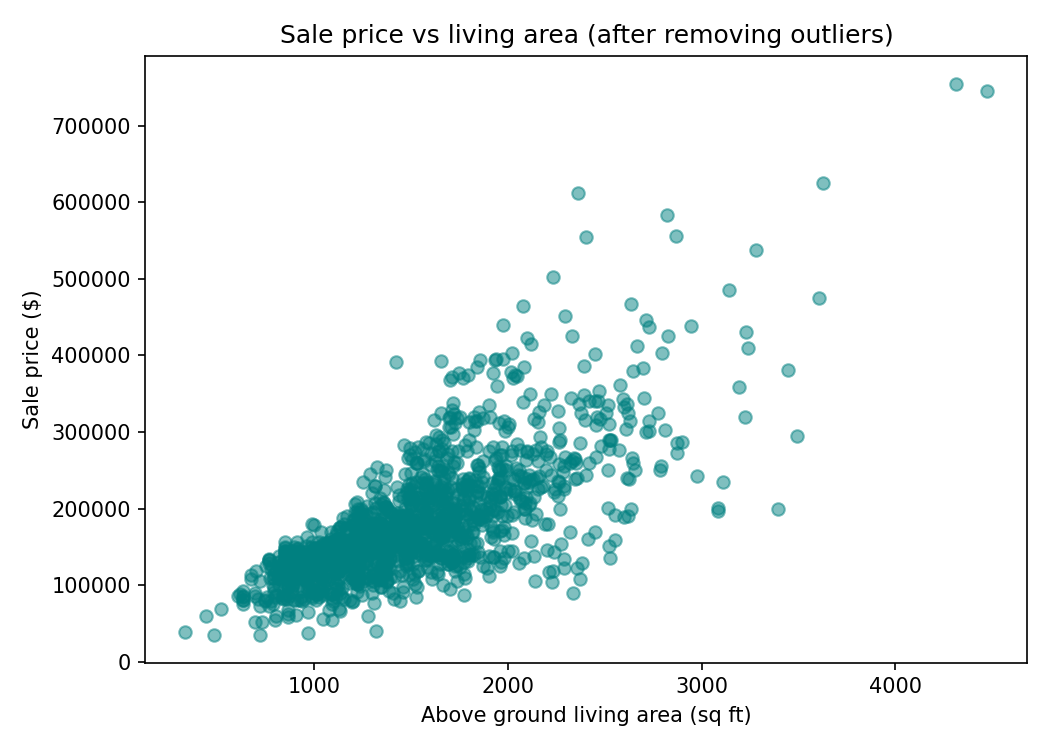
\includegraphics[width=0.65\textwidth]{fig_scatter_grlivarea.png}
    \caption{Sale price vs.\ living area, after removing outliers.}
    \label{fig:grlivarea-after}
\end{figure}

\subsection{Full list of columns with missing values}

\begin{table}[H]
    \centering
    \caption{All 19 columns with missing values before cleaning, and how each was handled.}
    \begin{tabular}{lrl}
        \toprule
        \textbf{Column} & \textbf{\% Missing} & \textbf{How it was handled} \\
        \midrule
        PoolQC       & 99.5\% & Filled with "None" \\
        MiscFeature  & 96.3\% & Filled with "None" \\
        Alley        & 93.8\% & Filled with "None" \\
        Fence        & 80.8\% & Filled with "None" \\
        MasVnrType   & 59.7\% & Filled with "None" \\
        FireplaceQu  & 47.3\% & Filled with "None" \\
        LotFrontage  & 17.7\% & Filled with per-neighborhood median \\
        GarageType   & 5.5\%  & Filled with "None" \\
        GarageYrBlt  & 5.5\%  & Filled with 0 \\
        GarageFinish & 5.5\%  & Filled with "None" \\
        GarageQual   & 5.5\%  & Filled with "None" \\
        GarageCond   & 5.5\%  & Filled with "None" \\
        BsmtFinType2 & 2.6\%  & Filled with "None" \\
        BsmtExposure & 2.6\%  & Filled with "None" \\
        BsmtFinType1 & 2.5\%  & Filled with "None" \\
        BsmtCond     & 2.5\%  & Filled with "None" \\
        BsmtQual     & 2.5\%  & Filled with "None" \\
        MasVnrArea   & 0.5\%  & Filled with 0 \\
        Electrical   & 0.1\%  & Filled with most common value \\
        \bottomrule
    \end{tabular}
\end{table}

\end{document}
